% Section explaining the theory governing the experiment

A compound pendulum (also known as a physical pendulum) consists of a \textbf{rigid} body oscillating about a pivot. This experiment uses a uniform metallic bar with holes/slots cut down the middle at regular intervals. The bar can be hung from any one of these holes allowing us to change the location of the pivot.

\section{Objective}

Derive an equation for the time period $T$ of the oscillations of a uniform metallic bar suspended from a pivot passing through it.

\section{Experimental Setup}

   The experimental equipment consists of a thin uniform metallic bar with holes/slots placed through it at regular intervals. By allowing the bar to swing from different slots one can change the Moment of Inertia and consequently the Time Period of oscillations.

   \begin{center}
      \tikzsetnextfilename{setup}
\begin{center}
   \begin{tikzpicture}

      \usetikzlibrary{patterns}
      % We define a tikz style which defines a fill pattern consisting of lines in the north east direction.
      % The draw=none option indicates that we do NOT want any stroke/border around the fill
      \tikzstyle{wall}=[fill,pattern=north east lines,minimum width=0.75cm,minimum height=0.3cm, draw=none]


      % Define dimensions and angles
      \def\hw{0.25}     % Half width of the small wall segment on top

      \def\angle{-120}  % Angle of string
      \def\r{5}         % Radius of string

      \def\br{0.1}      % Radius of bob


      % Draw commands
      \draw (-\hw, 0) -- (\hw, 0);
      \draw [wall] (-\hw,0) rectangle (\hw,0.1);        % Draws a rectangle using the 'wall' pattern giving us the sloped lines

      \draw (0,0) -- (\angle:\r);       % string
      \draw [dashed] (0,0) -- (0,-\r);  % Dashed line down the middle

      \draw (\angle:\r+\br) circle [radius=\br];
      
   \end{tikzpicture}
\end{center}
        % Include tex code for the diagram of the experimental setup
   \end{center}

   We define the total length of the bar as $L$ and the distance from the pivot to the center of mass (CM) of the bar to be $l$ as indicated in the diagram above. The position of the bar at any instant of time is given by the angle $\theta$. When allowed to swing the bar performs an approximation of simple harmonic motion, that is, the angle $\theta$ varies in a cyclic fashion with time period $T$.

\section{Free-Body Diagram}

To calculate the time period $T$ one has to derive the equation of motion $\theta(t)$, namely how the angle $\theta$ varies as a function of time $t$. The first step, as always, is drawing the extended free body diagram of the system (extended because we are dealing with a rotational system and therefore the distance from the pivot is significant).

   \begin{center}
      \tikzsetnextfilename{freebody}      % We set the filename which will be used for the pdf created by the externalize library. The prefix is still applicable so build/freebody.pdf will be created
\begin{center}
   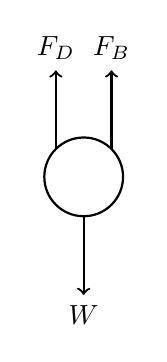
\begin{tikzpicture}

      \def\r{0.5}
      \def\h{1}

      \draw 
         (0,0) [thick] circle [radius=\r];

      \draw [thick] (0, -\r) [->] -- ++ (0,-\h) node [below] {$W$};

      \draw [thick] (45:\r) [->] -- ++ (0, \h) node [above] {$F_B$};

      \draw [thick] (135:\r) [->] -- ++ (0, \h) node [above] {$F_D$}; 

   \end{tikzpicture}
\end{center}

   \end{center}
